\section{Ánh xạ sang lược đồ CSDL}
Dựa trên phương pháp ánh xạ đã được học, nhóm sinh viên ánh xạ qua lược đồ cơ sở dữ liệu theo thứ tự sau:

\subsection{Bước 1: Ánh xạ các kiểu thực thể mạnh (Regular Entity Types)}
Thực thể mạnh bao gồm: \textbf{NGƯỜI DÙNG}, \textbf{KHÓA HỌC}, \textbf{CHƯƠNG}, \textbf{BÀI TẬP}, \textbf{BÀI KIỂM TRA}, \textbf{BÀI LUYỆN TẬP} và \textbf{BÀI VIẾT CHIA SẺ}. Tất nhiên các quan hệ dưới đây sẽ có thêm khóa ngoại khi chúng tham gia vào các mối liên kết mà sẽ được hoàn thiện ở các bước sau.
\begin{figure}[H]
    \centering
    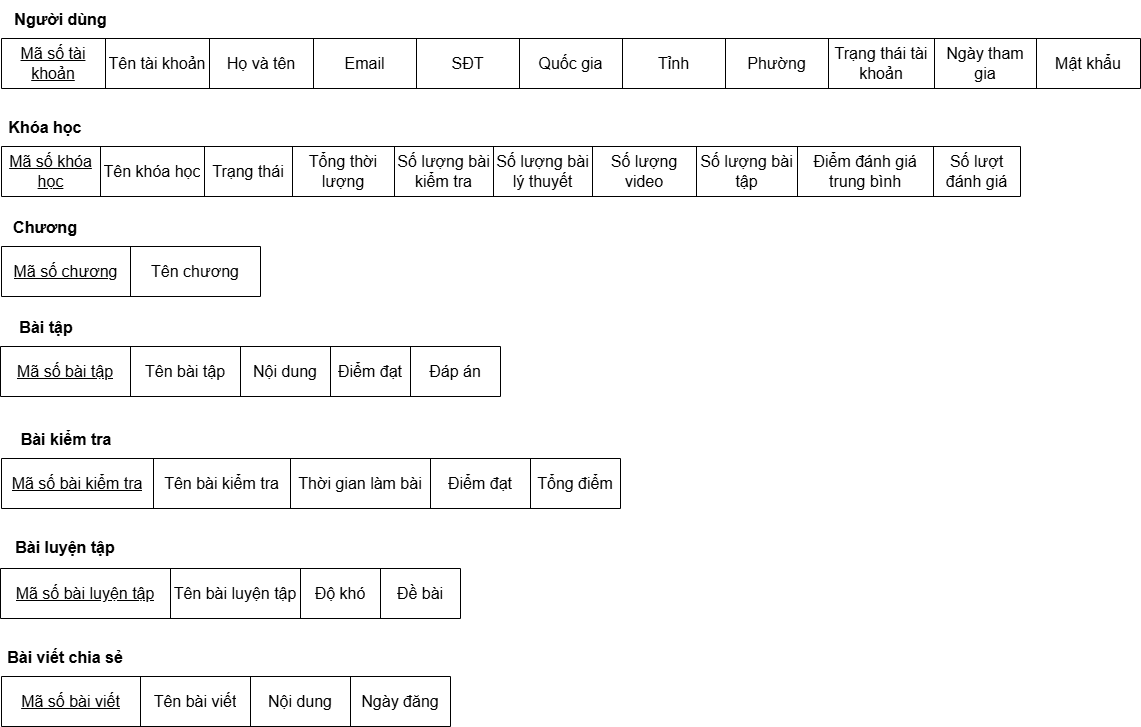
\includegraphics[width=1\linewidth]{picture/TTmanh.png}
    \caption{Bước 1: Ánh xạ các kiểu thực thể mạnh (Regular Entity Types)}
    \label{fig:placeholder}
\end{figure}
\subsection{Bước 2: Ánh xạ các kiểu thực thể yếu (Weak Entity Types)}
\textbf{BÌNH LUẬN} là thực thể yếu, khóa của thực thể này bao gồm cả khóa ngoại (Mã số tài khoản) và khóa riêng phần của chính nó (Thời gian).

\textbf{CÂU HỎI} là thực thể yếu, khóa của thực thể này bao gồm cả khóa ngoại (Mã số bài kiểm tra) và khóa riêng phần (STT).
\begin{figure}[H]
    \centering
    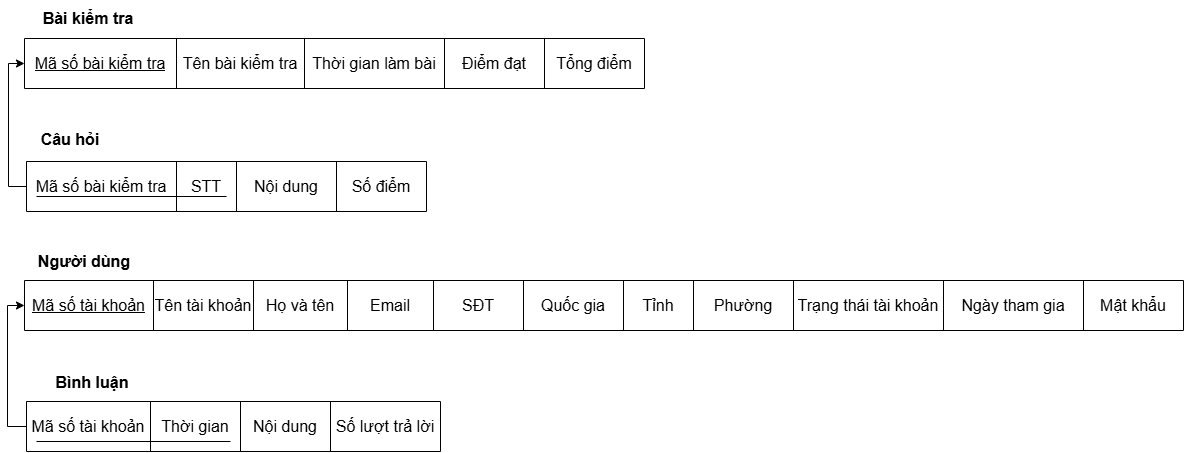
\includegraphics[width=1\linewidth]{picture/TTyeu.png}
    \caption{Bước 2: Ánh xạ các kiểu thực thể yếu (Weak Entity Types)}
    \label{fig:placeholder}
\end{figure}
\vspace{-20pt}
\subsection{Bước 3: Ánh xạ các kiểu mối liên kết hai ngôi 1:1 (Binary	1:1	Relationship Types)}
Mỗi \textbf{CHƯƠNG} có một \textbf{BÀI KIỂM TRA}, nên ta đưa khóa chính của \textbf{CHƯƠNG} vào làm  khóa ngoại của \textbf{BÀI KIỂM TRA} để thể hiện mối liên kết \textbf{có} 1:1. \vspace{-12pt}
\begin{figure}[H]
    \centering
    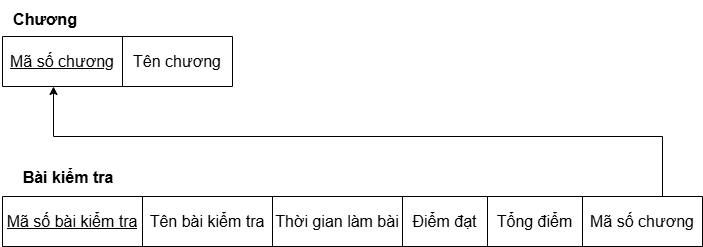
\includegraphics[width=0.75\linewidth]{picture/lk1-1.png}
    \caption{Bước 3: Ánh xạ các kiểu mối liên kết hai ngôi 1:1 (Binary	1:1	Relationship Types)}
    \label{fig:placeholder}
\end{figure}
\subsection{Bước 4: Ánh xạ các kiểu mối liên kết hai ngôi 1:N (Binary	1:N	Relationship Types)}
\textbf{NGƯỜI DÙNG} \textbf{đăng} \textbf{BÀI VIẾT},

\textbf{NGƯỜI DÙNG} \textbf{viết} \textbf{BÌNH LUẬN},

\textbf{GIÁO VIÊN} \textbf{tạo} \textbf{KHÓA HỌC},

\textbf{GIÁO VIÊN} \textbf{tạo} \textbf{BÀI LUYỆN TẬP},

\textbf{KHÓA HỌC} \textbf{có} \textbf{CHƯƠNG}, 

\textbf{KHÓA HỌC} \textbf{có} \textbf{BÌNH LUẬN},

\textbf{CHƯƠNG} \textbf{có} \textbf{BÀI TẬP},

\textbf{BÀI KIỂM TRA} \textbf{có} \textbf{CÂU HỎI},

\textbf{BÀI VIẾT CHIA SẺ} \textbf{có} \textbf{BÌNH LUẬN},

\textbf{BÌNH LUẬN} \textbf{có} \textbf{BÌNH LUẬN} khác phản hồi là các mối liên kết hai ngôi 1:N.
\begin{figure}[H]
    \centering
    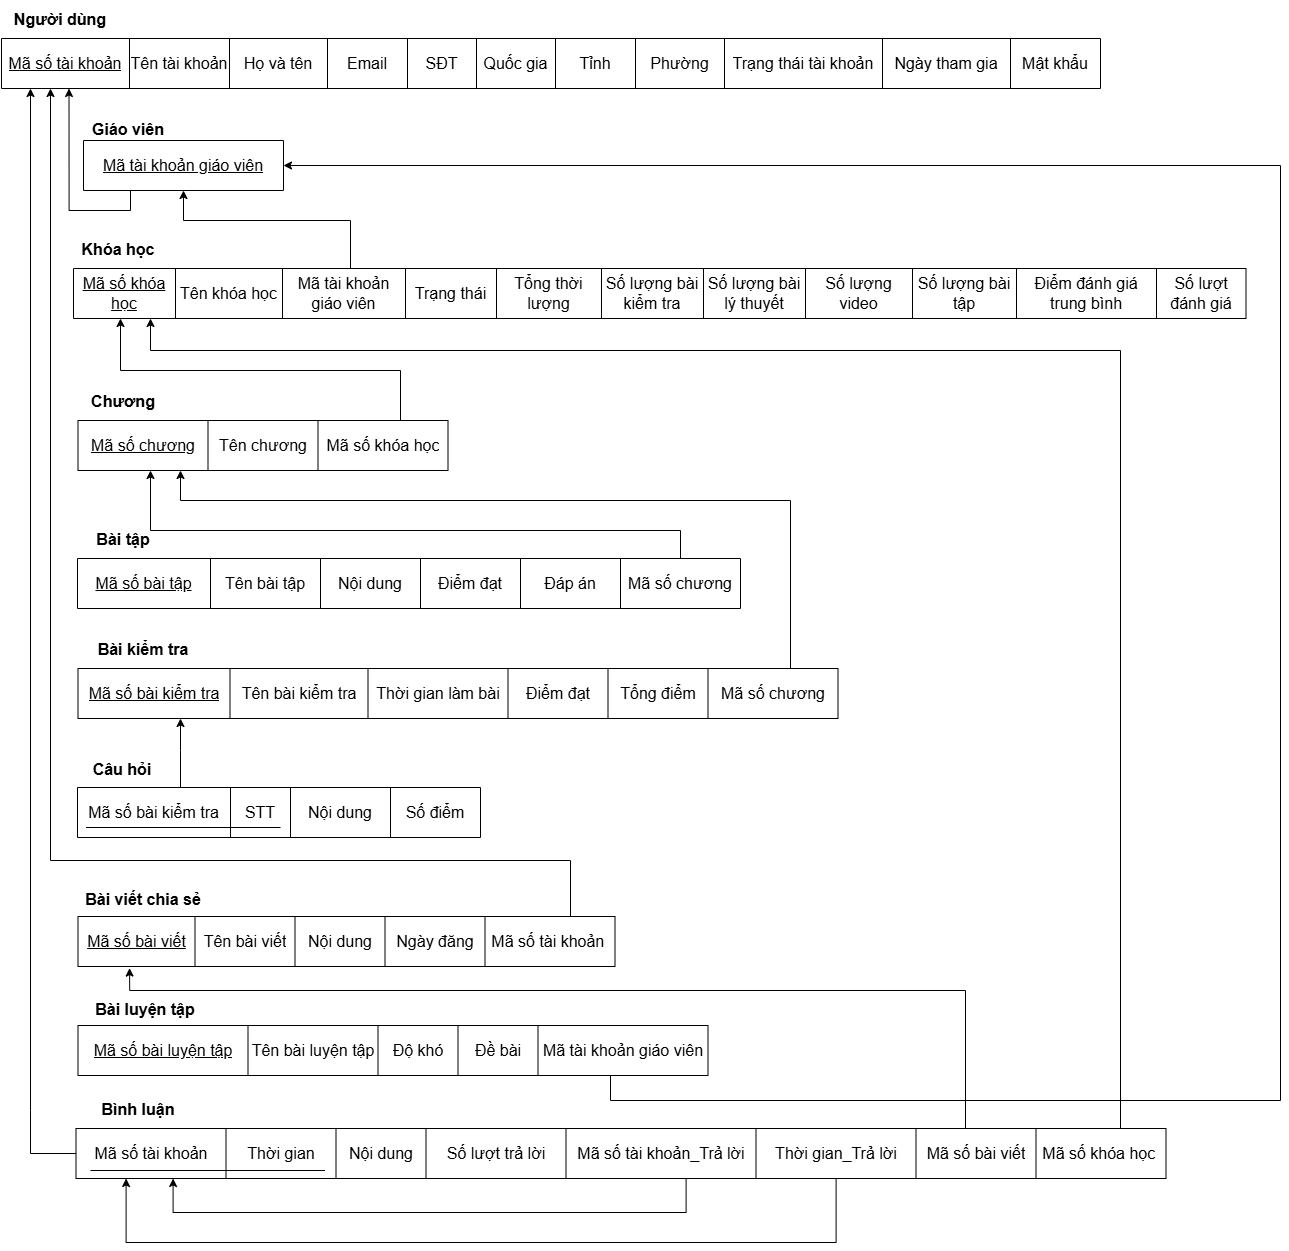
\includegraphics[width=1\linewidth]{picture/lk1-n.png}
    \caption{Bước 4: Ánh xạ các kiểu mối liên kết hai ngôi 1:N (Binary	1:N	Relationship Types)}
    \label{fig:placeholder}
\end{figure}
\vspace{-30pt}
\subsection{Bước 5: Ánh xạ các kiểu mối liên kết hai ngôi N:N (Binary	N:N	Relationship Types)}
\textbf{NGƯỜI DÙNG} \textbf{thực hiện} \textbf{BÀI KIỂM TRA}, 

\textbf{NGƯỜI DÙNG} \textbf{thực hiện} \textbf{BÀI TẬP},

\textbf{NGƯỜI DÙNG} \textbf{thực hiện} \textbf{BÀI LUYỆN TẬP},

\textbf{NGƯỜI DÙNG} \textbf{tham gia} \textbf{KHÓA HỌC},

\textbf{NGƯỜI DÙNG} \textbf{đánh giá} \textbf{KHÓA HỌC} là các mối liên kết hai ngôi N:N.
\begin{figure}[H]
    \centering
    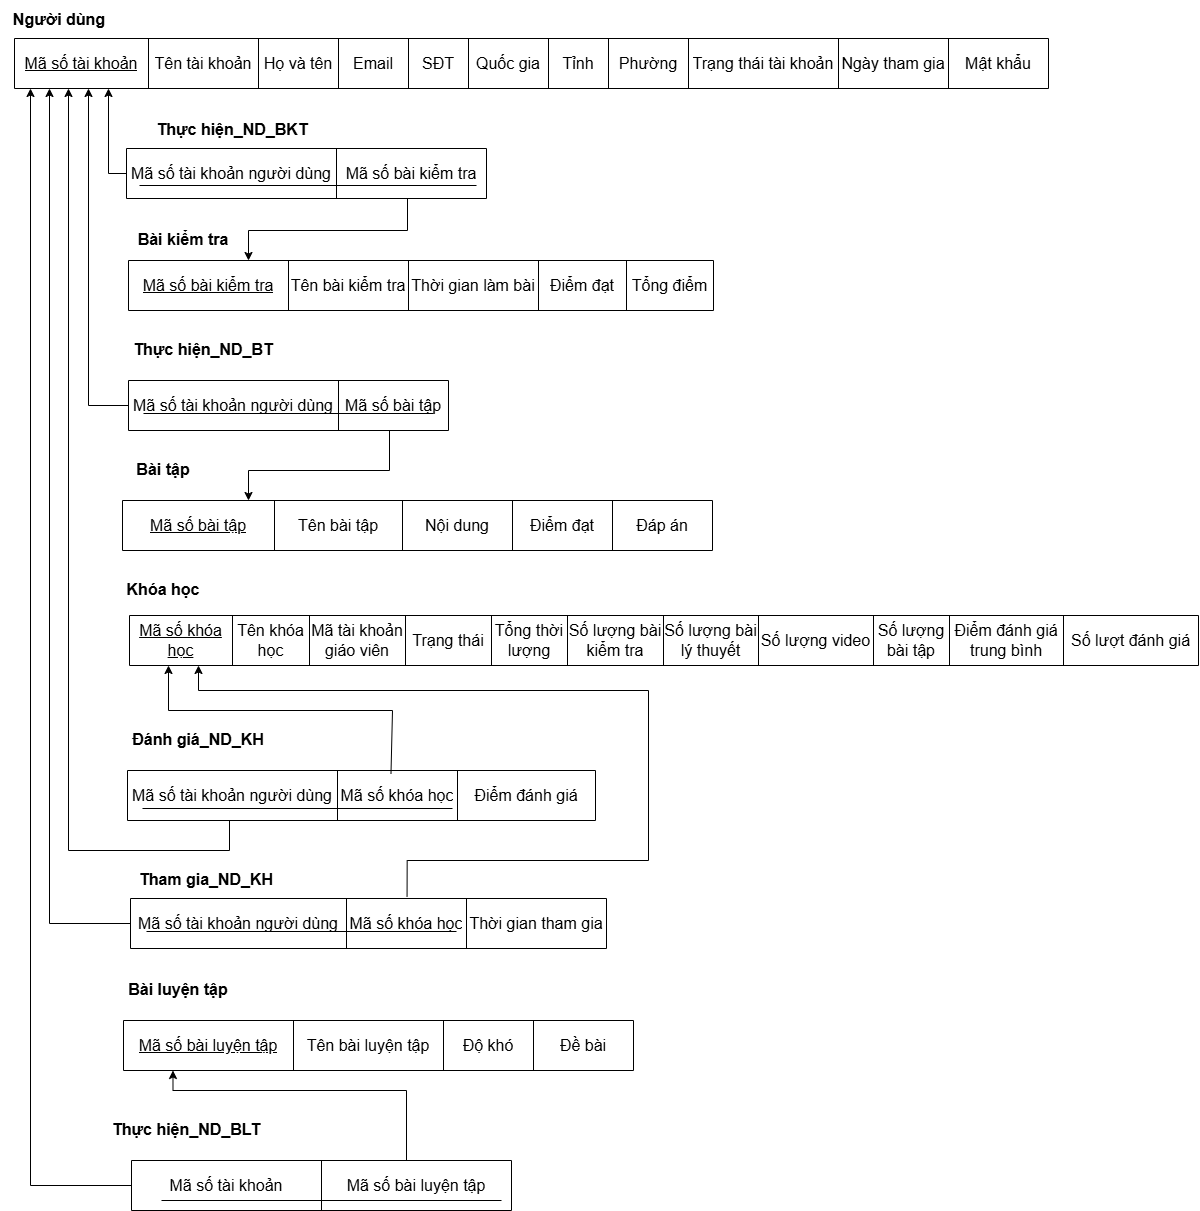
\includegraphics[width=1\linewidth]{picture/lkn-n.png}
    \caption{Bước 5: Ánh xạ các kiểu mối liên kết hai ngôi N:N (Binary	N:N	Relationship Types)}
    \label{fig:placeholder}
\end{figure}
\vspace{-40pt}
\subsection{Bước 6: Ánh xạ các thuộc tính đa trị (Multivalued	attributes)} \vspace{-4pt}
Các thuộc tính đa trị gồm: Video bài học, Bài học lý thuyết của \textbf{CHƯƠNG}, Ghi nhận thực hiện của mối liên kết \textbf{NGƯỜI DÙNG thực hiện BÀI TẬP}, Ghi nhận thực hiện của mối liên kết \textbf{NGƯỜI DÙNG thực hiện BÀI KIỂM TRA}, Học vấn của \textbf{GIÁO VIÊN}, Thông tin làm bài luyện tập của mối liên kết \textbf{NGƯỜI DÙNG thực hiện BÀI LUYỆN TẬP}.
\begin{figure}[H]
    \centering
    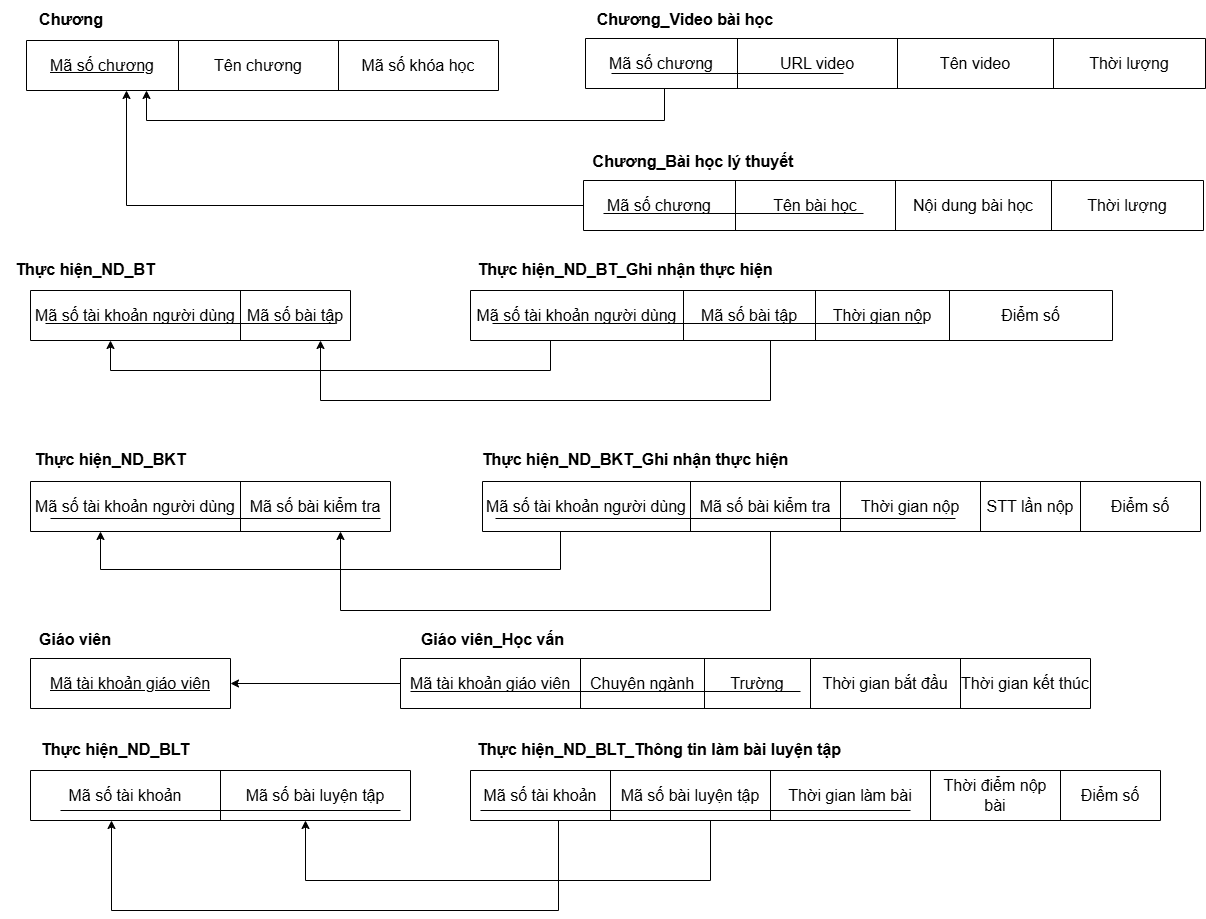
\includegraphics[width=1\linewidth]{picture/datri.png}
    \caption{Bước 6: Ánh xạ các thuộc tính đa trị (Multivalued	attributes)}
    \label{fig:placeholder}
\end{figure}
\subsection{Bước 7: Ánh xạ chuyên biệt hóa (lớp cha – lớp con)}
Lớp \textbf{NGƯỜI DÙNG} có lớp con là \textbf{GIÁO VIÊN}.
\begin{figure}[H]
    \centering
    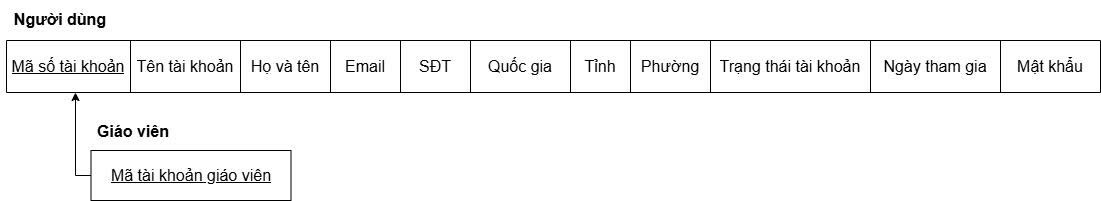
\includegraphics[width=1\linewidth]{picture/chacon.jpg}
    \caption{Bước 7: Ánh xạ chuyên biệt hóa (lớp cha – lớp con)}
    \label{fig:placeholder}
\end{figure}